\chapter{User Manual}
\thispagestyle{fancy}

To quickly have a look at what was realized during the semester thesis, just 
install the \textit{Toggle Function Definition} code automation according to 
this manual.

\section{Installation of the plugin}

To try out the plugin, you will need a running Eclipse Helios (3.6) installation with CDT already installed. Choose "Help", "Install New Software..." and type in the following url into the address bar:

\url{http://sinv-56042.edu.hsr.ch/updatesite}

The plugin may now be installed using the install wizard. Be aware that the 
update site is hosted on a virtual server that will be removed at the end of 
summer 2011. However, a copy of the whole virtual server may be found on the 
attached DVD.
% TODO: really attach a DVD at the end of the project...

\subsection{Activate the menu item}

\begin{figure}[h]
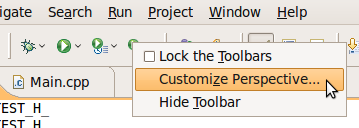
\includegraphics[width=0.4\textwidth]{images/customizeperspective.png}
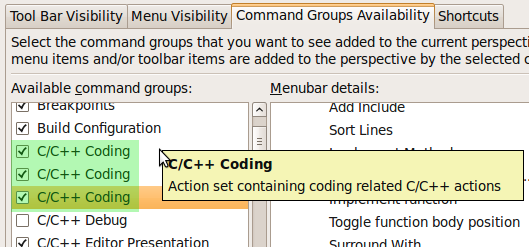
\includegraphics[width=0.6\textwidth]{images/commandgroups.png}
\caption{To use the refactoring from the menu, it needs to be enabled manually 
after installation.}
\label{showMenu}
\end{figure}
\label{cmdGroup}
To run the refactoring using the menu, some changes have to be applied to the 
current perspective. Right-click on the toolbar and choose 
"Customize perspective...". Then go to the "Groups and commands visibility" tab 
and check \textbf{all} "C++ coding" boxes. The menu "Toggle Function Definition" 
should now be visible inside the source menu.

\section{Use of the \textit{Toggle Function Definition} refactoring}

The refactoring may be applied as soon as the cursor is placed inside a function that is well defined. The definition may 

\section{Example}

The following graphics show an example workflow with the \textit{toggle 
refactoring}. Figure \ref{exampleA} shows what happens to a regular member 
function that was previously defined inside its class definition when the toggle 
refactoring is invoked on it. The implementation of the member function 
\textit{move} becomes separated from the class definition.

\begin{figure}[h]
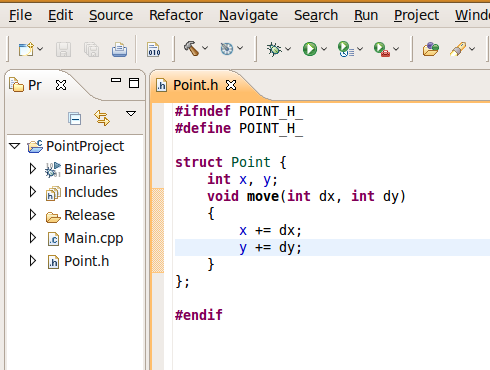
\includegraphics[width=0.5\textwidth]{images/step1.png}
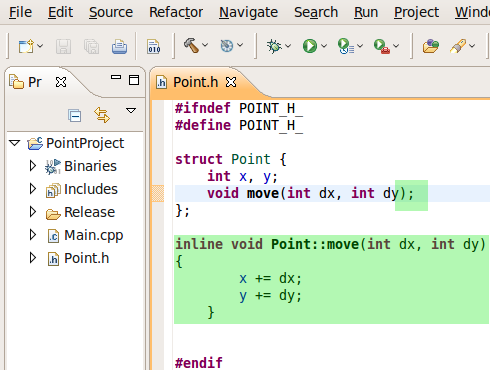
\includegraphics[width=0.5\textwidth]{images/step2.png}
\caption{initial situation and situation after first toggling}
\label{exampleA}
\end{figure}

When no source file exists that includes the header file, the user is asked 
whether he wishes to move the function to a new source file named 
\textit{Point.cpp} as shown in figure \ref{exampleB}.

\begin{figure}[h]
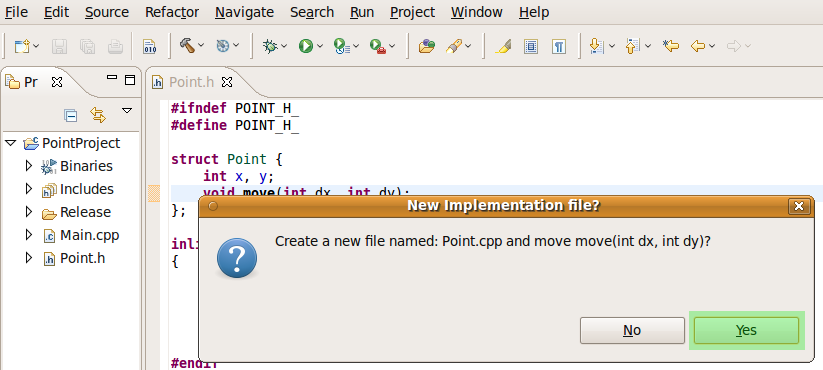
\includegraphics[width=\textwidth]{images/step3a.png}
\caption{ask to create a new source file if none was found}
\label{exampleB}
\end{figure}

The source file now got created. Function definition and declaration are 
splitted up into two separate files. The function definition may now be toggled 
back again into the class definition.

\begin{figure}[h]
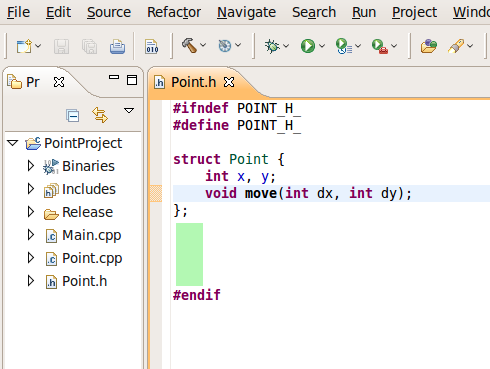
\includegraphics[width=0.5\textwidth]{images/step3b.png}
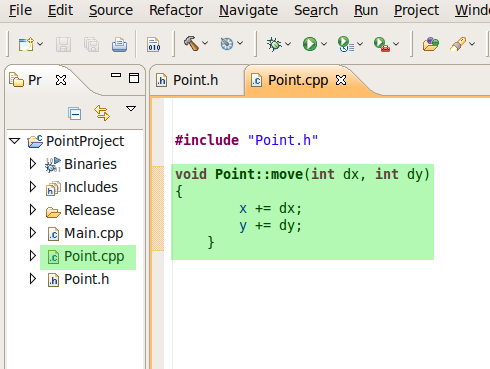
\includegraphics[width=0.5\textwidth]{images/step3c.png}
\caption{situation after second toggle: Point.cpp newly created}
\label{exampleC}
\end{figure}

